\subsection{User Submitted Content}
To improve the relevance and the features of the balloon news system, it was decided that consumers should be allowed to generate their own content. This content would be news articles and pictures from the internet which would then be sent along with the twitter feed to the balloon news feed to be displayed on the screen, represented by a balloon.

A series of requirements were then drawn up for what was wanted for user generated content to work. It was decided that user should be able to give an article, a picture to represent that and an excerpt. The picture and excerpt would be shown on the main screen of the application to entice users to read the article. The balloon customization allows the user to be able to easily identify their balloon. Note that this system is separate from the service that passes the information over to the balloons, though this service will use the same database.

The requirements are as follows:

\begin{itemize}
\item{Allow the user to submit a website to the application}
\item{Save the information on who submitted it, the content of the website and a picture that represents the article}
\item{Allow this information to be passed to the screens running the balloon news application along with the twitter feed}
\item{Allow the user to set the balloon colour of the balloon to carry their news}
\item{Allow the user to upload a picture to represent their article}
\item{Allow the user to give an excerpt of the article as a summary of what the article is about}
\item{Let an administrator be able to remove articles if they are found to be offensive or inadequate}
\end{itemize}

\subsection{Design}
It was very obvious from the beginning that trying to submit an article using the screens and the Kinect interface was going to present a problem. It was therefore decided that a website should be built for the user to perform this process. This would allow them more flexibility and the more familiar interface of the mouse and keyboard.

It was decided that the technologies that should be used were a website built with HTML, CSS and JavaScript with a PHP backend supported by a MySQL database. This was due to the programmers having a good knowledge of PHP and that it fitted well technologically with the system it was being designed for. Most of the processing would therefore be done server side with the website being a simple way for the user to submit and retrieve information.

To speed up the development of the backend a PHP framework was decided upon. CodeIgniter was the chosen PHP framework because it was easy to set up, had a lot of features and good community support.

\subsection{Website Design}
The website consisted of three main pages, one for viewing content that had been submitted, one for logging in to the system and another for submitted content to the website. These three pages covered the requirements of the system and were done in a way that made the website easy to use. 

\subsubsection{Header}
All pages are given the same header (figure \ref{Website-Header}). This kept the design consistent throughout the website which makes it easier for users to navigate around it and find what they want.

\begin{figure}
\begin{centering}

\includegraphics[width=\textwidth]{Diagrams/Website-Header}
\par\end{centering}

\caption{Website Header}
\label{Website-Header}
\end{figure}

It has the Heriot-Watt logo in the top left corner so users knew it is associated with the university. It then has the title of the website and a logged in status. To the right of that are the links to each part of the website. The header is made to be simple and clear. The links are easily identified by their different colour which mimics other typical hyperlink colours. The user can easily take in all this information very quickly.

\subsubsection{Content Viewer}
This page (see figure \ref{ContentViewer}) is the main page of the website and the starting point. Its aim is to show users what content is appearing on the balloons right now. It currently shows up to 10 items with all the information submitted such as the article URL, balloon colour and article title.

\begin{figure}
\begin{centering}
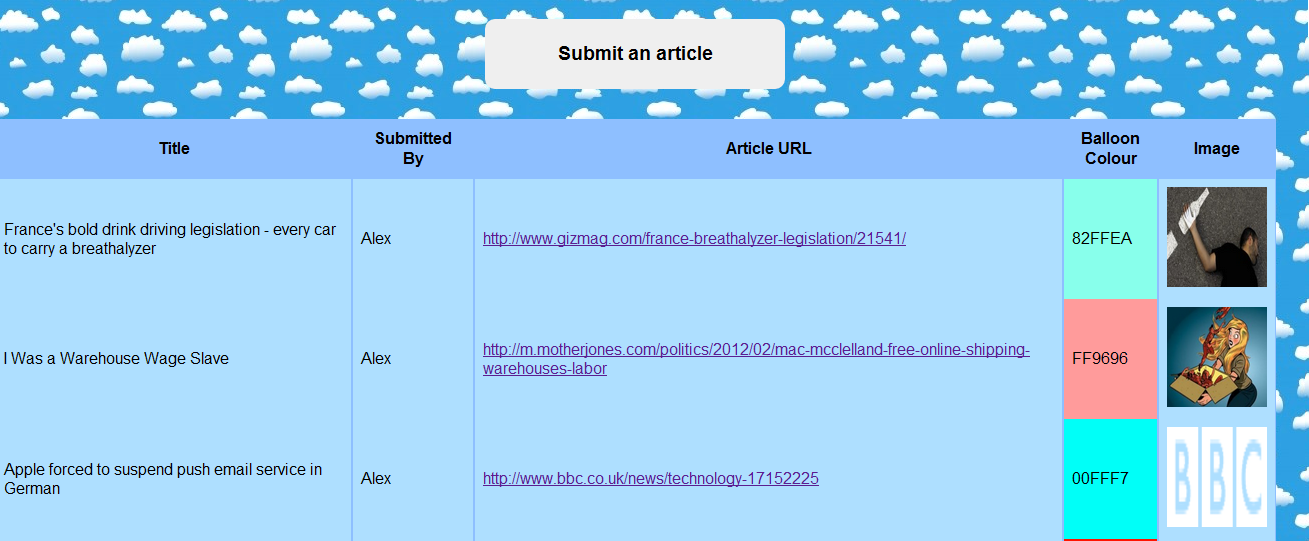
\includegraphics[width=\textwidth]{Diagrams/Website-ContentViewer}
\par\end{centering}

\caption{Content Viewer}
\label{ContentViewer}
\end{figure}

At the top of the page is an easy to access submit article button which clearly indicates that users can use this to add to the list of articles down below. The table below that gives information on the articles submitted. Where applicable an image or colour is shown to better show what has been submitted.

The system can be made to allow some users to be administrators. This is currently based on group ID when they are logged in. If they are of group users or staff then they have admin rights. Most students have a group ID of cs4 or some other representation of their course. If an admin user is logged in then they will be able to remove content they find offensive or not suitable. They can do this via an extra remove field in the table (see figure \ref{RemoveContent}).

\begin{figure}
\begin{centering}
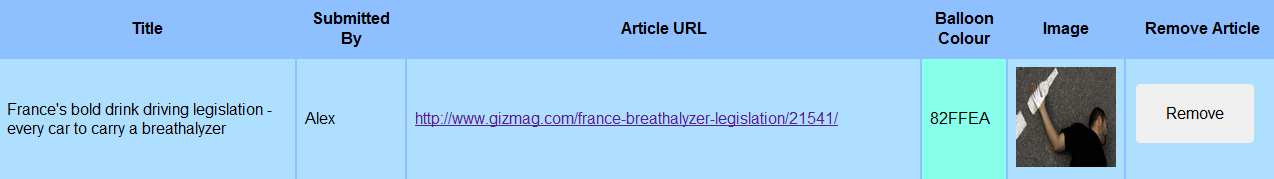
\includegraphics[width=\textwidth]{Diagrams/Website-RemoveContent}
\par\end{centering}

\caption{Content Removal By Administrators}
\label{RemoveContent}
\end{figure}

\subsubsection{Login Page}
The login page (see figure \ref{Login}) enables the user to enter the submission process of the website. A user cannot access the article submission page without logging in. 

\begin{figure}
\begin{centering}
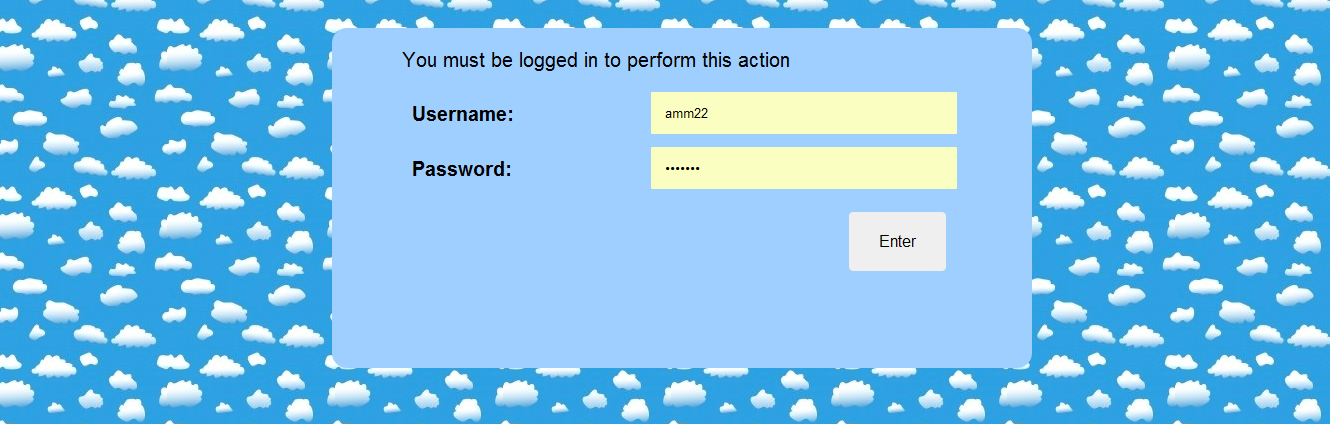
\includegraphics[width=\textwidth]{Diagrams/Website-Login}
\par\end{centering}

\caption{Login Page}
\label{Login}
\end{figure}

The page is very simple. The user has to enter their username and their password. The username and password used are the ones for the MACS system. A user cannot use this website if they are not a member of the MACS network. 

\subsubsection{Article Submission Page}
The final page in the website is the one for submitting articles (see figure \ref{ContentSubmission}). This had to be simple to use and clear. It was therefore made to have large text entry points and clear labels.

\begin{figure}
\begin{centering}
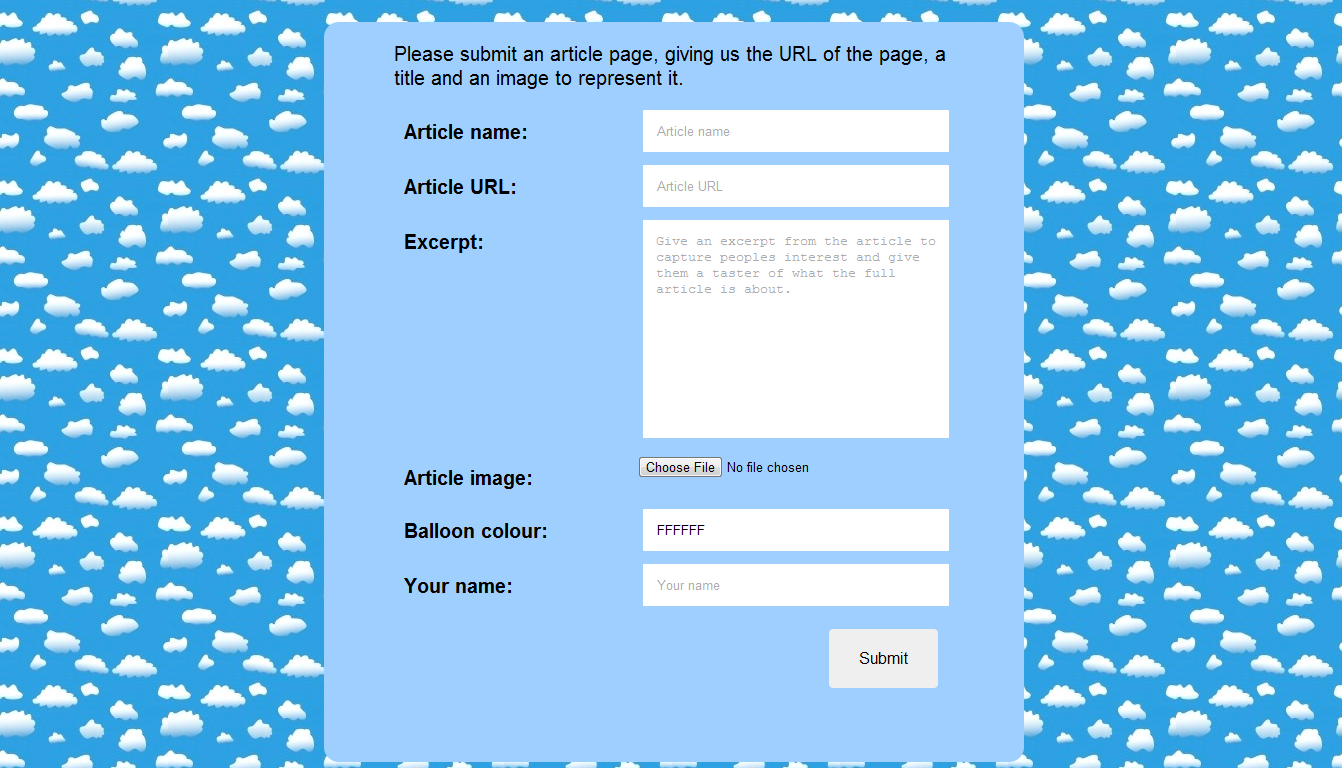
\includegraphics[width=\textwidth]{Diagrams/Website-Submission}
\par\end{centering}

\caption{Content Submission}
\label{ContentSubmission}
\end{figure}

The user is asked to submit a title, URL and Excerpt from their article. These can be copied and pasted from the article webpage itself. An image can then be uploaded that would represent the article. This could also come from the article but would have to be saved on the local machine first. Next the user enters their balloon colour using a user friendly colour selector and then puts in some alias for them. 

The submit button is located on the bottom right as is usual for a culture that reads from left to right, top to bottom. This makes it very clear to the user how to finish uploading their content. When a user clicks this button the submission will either fail or succeed. If it fails they are given a message in read up above the article name field. If it is successful then they are taken to the article viewer page and given a message that their submission was successful. They will also be able to see their submission.

\subsection{Article Submission Page}
The database would be used by the part of the system responsible for sending news feed information to the screens. The article itself would have to be stored as a URL, this could them be retrieved from the database and used to either render the page or be provided to the users via a QR code for them to lookup on their mobile phone. Storing the article itself would have taken up too much space and been unnecessary. The picture to represent the article would also be stored as a URL. This would allow us to host it on our web space, 
thereby saving more space in our database. 

The database schema was therefore as follows: 

\singlespacing
\begin{verbatim}ContentID	BIGINT UNSIGNED NOT NULL AUTO_INCREMENT
Title		VARCHAR (255)
SubmittedBy	VARCHAR (10)
URL		VARCHAR (255)
Excerpt		MEDIUMTEXT
TimeCreated	TIMESTAMP DEFAULT CURRENT_TIMESTAMP
BalloonColour	CHAR (6) DEFAULT FFFFFF
ImageURL	VARCHAR (255)
Votes		INT (11) DEFAULT 0
GivenName	VARCHAR (50)\end{verbatim}
\onehalfspacing

This gives the system all the information it needs to send information on news articles to the feed. The content ID is just a primary key to identify each row. The title, excerpt and URL are all information on the article to submit. The image is stored as a URL which points to a location on the systems web space. Information on the user is also stored. For reasons of privacy the user can specify which name they wish to be known by, however their real user ID is recorded too in the submitted by field.

\subsection{Website Code Structure}
The structure was based on CodeIgniter's structure. CodeIgniter has a strong Model, View, Controller set up so it would make code clearer and more modular. The overall layout of the website will now be looked at and then the main sections will be covered in depth. This will start with the folder structure of CodeIgniter (Only important folders shown). Note that this backend was also used for deploying the balloon content to screens, though that will be covered later.

\singlespacing
\begin{verbatim}application/
    config/
    controllers/
    models/
    views/
included/
uploads/\end{verbatim}
\onehalfspacing

These are the main directories that have been modified. There are several other directories but they just contain base CodeIgniter functionality which is not important here. The application folder contains all the PHP scripts required to create the website. This is where all the development is done. The included folder stores any CSS, JavaScript and additional pictures or material for design. Uploads is where the pictures are stored for use with the balloons. This allows the screen easy access to the pictures by getting them from this folder and saves space in the database.

Within the application folder are the files that are most important. The config folder contains settings for the website to work correctly. For example the base\_url stores the basic URL to the website as seen from someone accessing it remotely. This will need to be changed when installing it on another server.

The controllers folder contains the entry point for different parts of the application. For example the login page is controlled by the login controller. For more information on the model view controller architecture see \url{http://en.wikipedia.org/wiki/Model\%E2\%80\%93view\%E2\%80\%93controller}. There are three controllers for the content submission part of this website. These are the welcome.php which handles the login page and the functionality of users logging in, content\_manager.php which handles the displaying and removing of content from the database and finally submit\_content.php which handles the submission form and submission of news articles.

The models folder contains classes for interacting with the database and any other I/O that has to happen. There are just two models, one for users and one for content. The users model is for checking for valid users against MACS user database using the Linux getpwnam command. This encrypts the password the user provides and checks it against the encrypted form on the MACS network. The content model interacts with the database which stores content. It performs functions such as adding, getting and removing content from the database.

The views folder contains all the HTML pages that get sent to the user. Each of these pages is called by a controller so there are three views. One for logging in, one for displaying content and finally one for letting users submit content. To create the header there is an includes folder. The includes folder contains a template, header and footer. The template is a view that loads the header, main page and footer onto one page. The header and footer are just HTML pages that contain that start and end of the web page. None of the main pages therefore have the HTML tags or HEAD tags. 
